\documentclass{article}
\usepackage[utf8]{inputenc}
\usepackage{graphicx}
\usepackage{wrapfig}
\usepackage{array}
\usepackage{siunitx}
\usepackage{xcolor}
\usepackage{multicol}
\usepackage{amssymb}
\setlength{\columnseprule}{1pt}

\title{Time Constant of a Capacitor and Step Response in RLC Circuits \\ Lab Report 3 \\ ELP100}
\author{Yash Agarwal \\ 2021EE10638 \\ Group 29}
\date{May 04, 2022}

\begin{document}
\pagecolor{yellow!15}
\maketitle
\vspace{15px}
\tableofcontents
\newcolumntype{V}{>{\centering\arraybackslash} m{.4\linewidth} }
\newpage
\section{Time Constant in RC Circuit}
\subsection{Aim}
To observe and trace the complete response to step input and to determine the time constant and check with the theoretically calculated value. 
\subsection{Apparatus}
\begin{enumerate}
\item Breadboard and Jumpers
\item Variable resistor and Multimeter
\item Capacitor of capacitance – 0.22 $\mu$F
\item Digital Storage Oscilloscope (DSO1052B)
\item Function Generator (0 – 3 MHz)
\end{enumerate}

\subsection{Theory}

\begin{wrapfigure}{R}{0.3\textwidth}
\fcolorbox{black}{white}{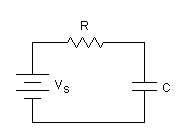
\includegraphics[width=0.25\textwidth]{RC Circuit.png}}
\end{wrapfigure}

To find the complete response of an RC Series Circuit, we find the zero input response (Natural Response) and zero state response (Forced Response), and then add them together.

\noindent
Natural Response: \[ C\times\frac{dV_c}{dt}+\frac{v_c}{R}=0\]
In case of Charging, the Solution is $V_c=V_0(1-e^{-\frac{t}{RC}})$ where RC is known as Time Constant.\\
\noindent
In case of Discharging, the Solution is $V_c=V_0e^{-\frac{t}{RC}}$ where RC is known as Time Constant.

\subsection{Breadboard Setup}
\vspace{5px}

\begin{multicols}{2}
\begin{center}
\fcolorbox{black}{white}{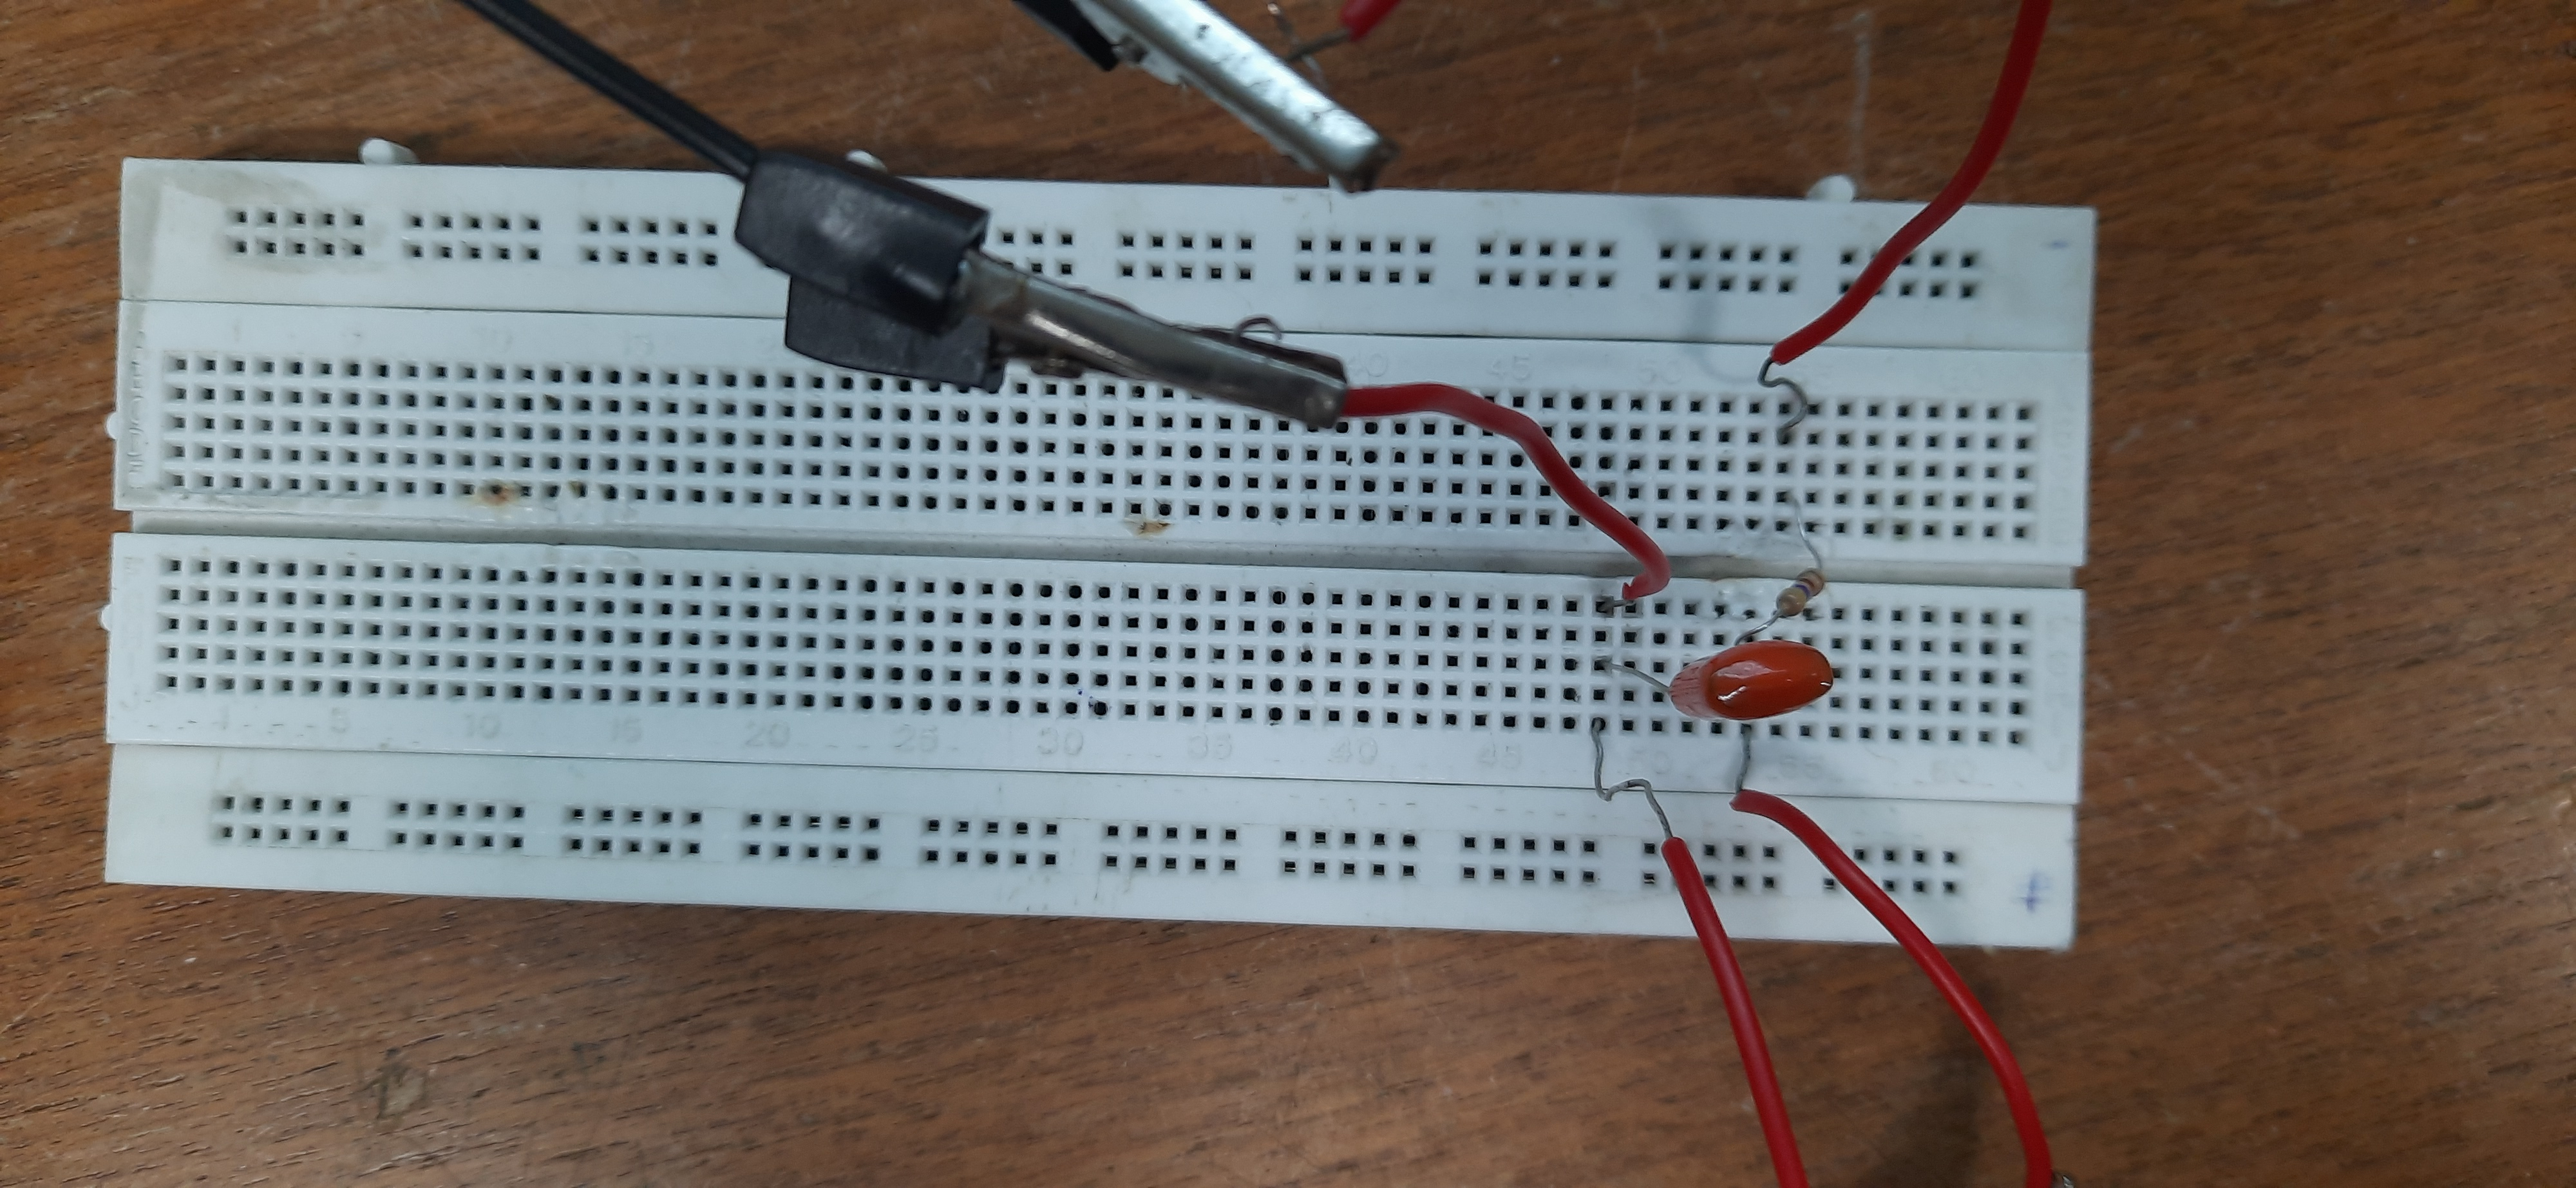
\includegraphics[width=0.9\columnwidth, height=100px]{CircuitRC.jpg}} \\ \vspace{5px}
Circuit with $R=470 \Omega$ and $C= 0.23 \mu F$ \\

\columnbreak

\fcolorbox{black}{white}{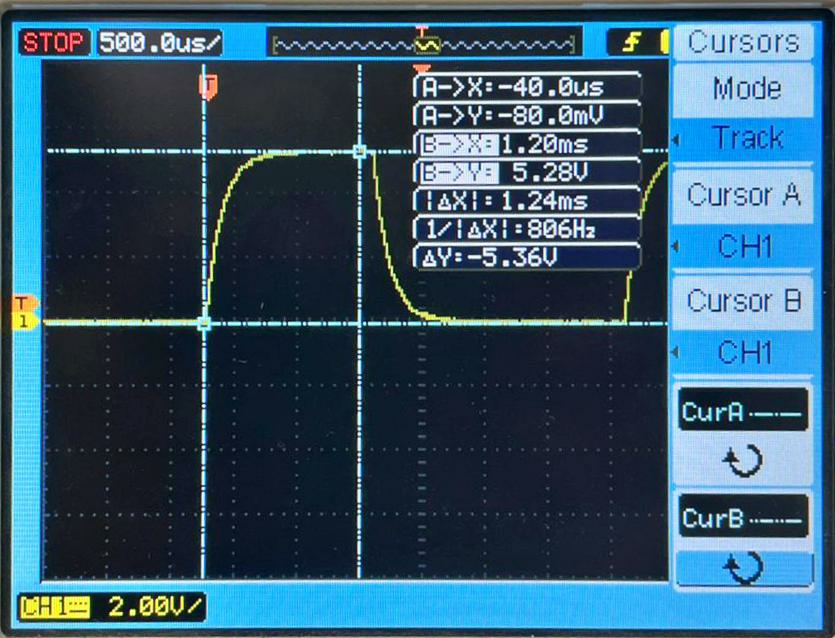
\includegraphics[width=0.9\columnwidth, height=100px]{Peak.jpeg}} \\ \vspace{5px}
Peak Voltage is 5.28V
\end{center}
\end{multicols}

\subsection{Observation}
\vspace{5px}
\begin{center}
\begin{tabular}{|c | c | c |} 
 \hline
    \ & \ & \ \\
    Case & Voltage ($V_\tau$) & Time Constant($\tau$) \\ [1em]
    \hline
    \ & \ & \ \\
    Charging & $63\% \ of \ 5.28=3.33$ & $132\mu s$  \\
    Discharging & $37\% \ of \ 5.28=1.94$ & $134\mu s$  \\
    \ & \ & \ \\
 \hline
\end{tabular}
\end{center}
\vspace{10px}
\begin{multicols}{2}
\begin{center}
\fcolorbox{black}{white}{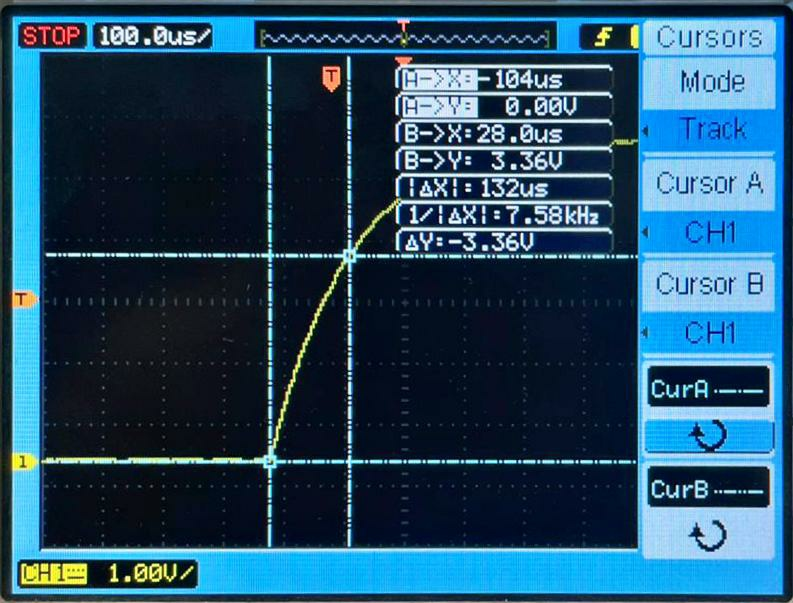
\includegraphics[width=0.9\columnwidth, height=100px]{Charging.jpeg}} \\ \vspace{5px}
Charging \\

\columnbreak

\fcolorbox{black}{white}{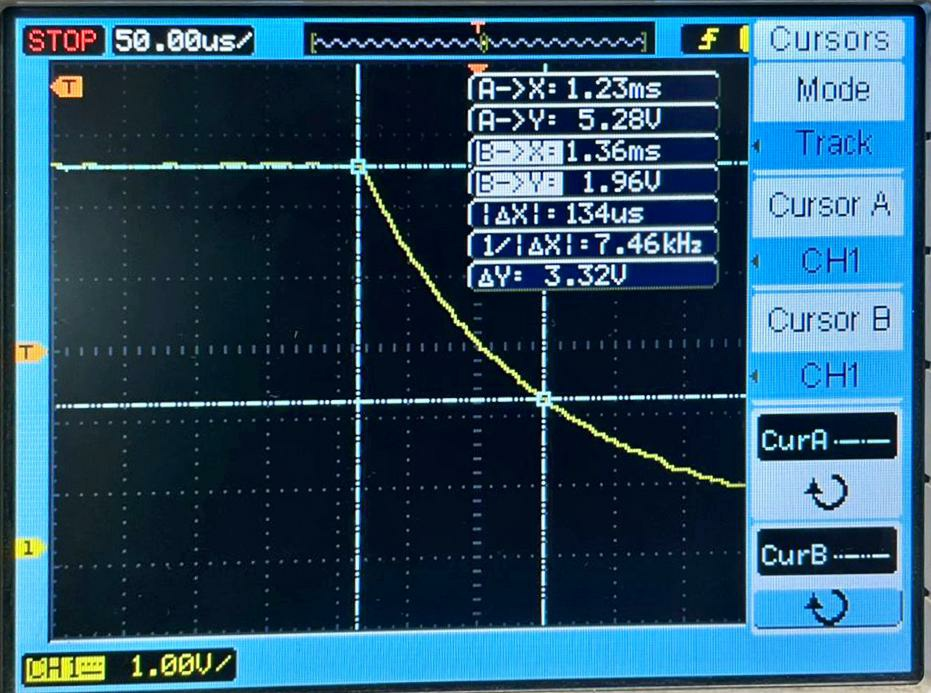
\includegraphics[width=0.9\columnwidth, height=100px]{Discharging.jpeg}} \\ \vspace{5px}
Discharging
\end{center}
\end{multicols}

\vspace{10px}

\subsection{Calculation}

Theoretical Time Constant ($\tau$) = $R\times C= 470\times0.23\times10^{-6}s$=108.1 $\mu s$

\noindent
Calculated Time Constant $\approx 133 \mu s$
\vspace{5px}

\subsection{Error Analysis}
Error= 133$ \mu s$ - 108.1$ \mu s$ = 24.9 $\mu s$

\noindent
Percentage Error= $ \frac{24.9}{133}$ $\times$ 100 = 18.7\%

\subsection{Conclusion}
Hence, within experimental error, we were able to measure the time constant of the series RC circuit with the help of a DSO machine.
\newpage

\section{Step Response in RLC Circuit}
\vspace{5px}
\subsection{Aim}
To observe and trace the complete response to step input in RLC Circuit
\vspace{5px}
\subsection{Apparatus}
\begin{enumerate}
\item Breadboard and Jumpers
\item Variable resistor and Multimeter
\item Capacitor of capacitance – 0.22 $\mu$F and Inductance of 2H
\item Digital Storage Oscilloscope (DSO1052B)
\item Function Generator (0 – 3 MHz)
\end{enumerate}
\vspace{5px}
\subsection{Theory}
\vspace{5px}
The general Solution of Voltage in Series RLC Circuit is of the form:
\[ A_1e^{-s_1t}+A_2e^{-s_2t} \]

\noindent
Where $s_1$ and $s_2$ are solutions of the Quadratic Equation:
\[ s^2+ 2\alpha s + \omega_0^2=0 \ where \ \alpha=\frac{R}{2L} \ and \ \omega_0^2=\frac{1}{LC} \] 

\noindent
Now we have 3 cases depending on the roots of the Quadratic:
\begin{enumerate}
    \item If $\alpha=\omega_0$ then roots are real and equal and circuit is Critically Damped
    \item If $\alpha>\omega_0$ then roots are real and distinct and circuit is Over Damped
    \item If $\alpha<\omega_0$ then roots are complex conjugates and circuit is Under Damped
\end{enumerate}

\begin{multicols}{2}
\begin{center}
\fcolorbox{black}{white}{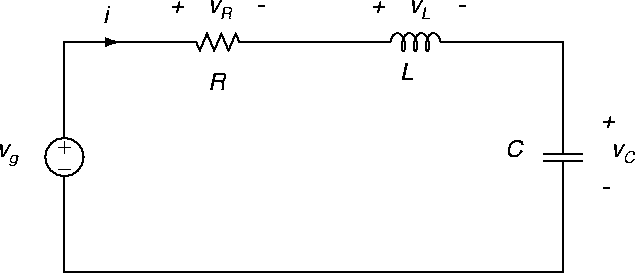
\includegraphics[width=0.9\columnwidth, height=100px]{RLC.png}} \\ \vspace{5px}
RLC Series Circuit \\

\columnbreak

\fcolorbox{black}{white}{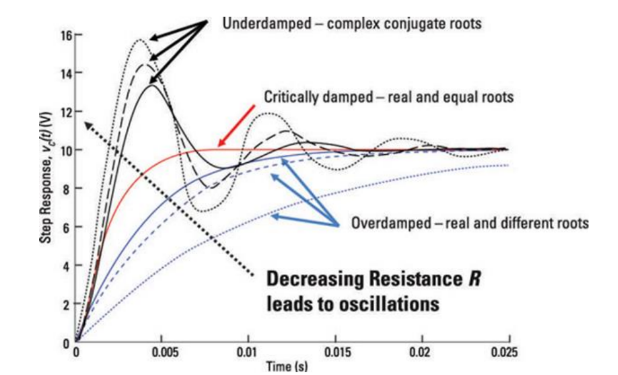
\includegraphics[width=0.9\columnwidth, height=100px]{Graph.png}} \\ \vspace{5px}
Effect of Changing Resistance on damping
\end{center}
\end{multicols}

\newpage

\subsection{Breadboard}
\vspace{10px}
\begin{center}
\fcolorbox{black}{white}{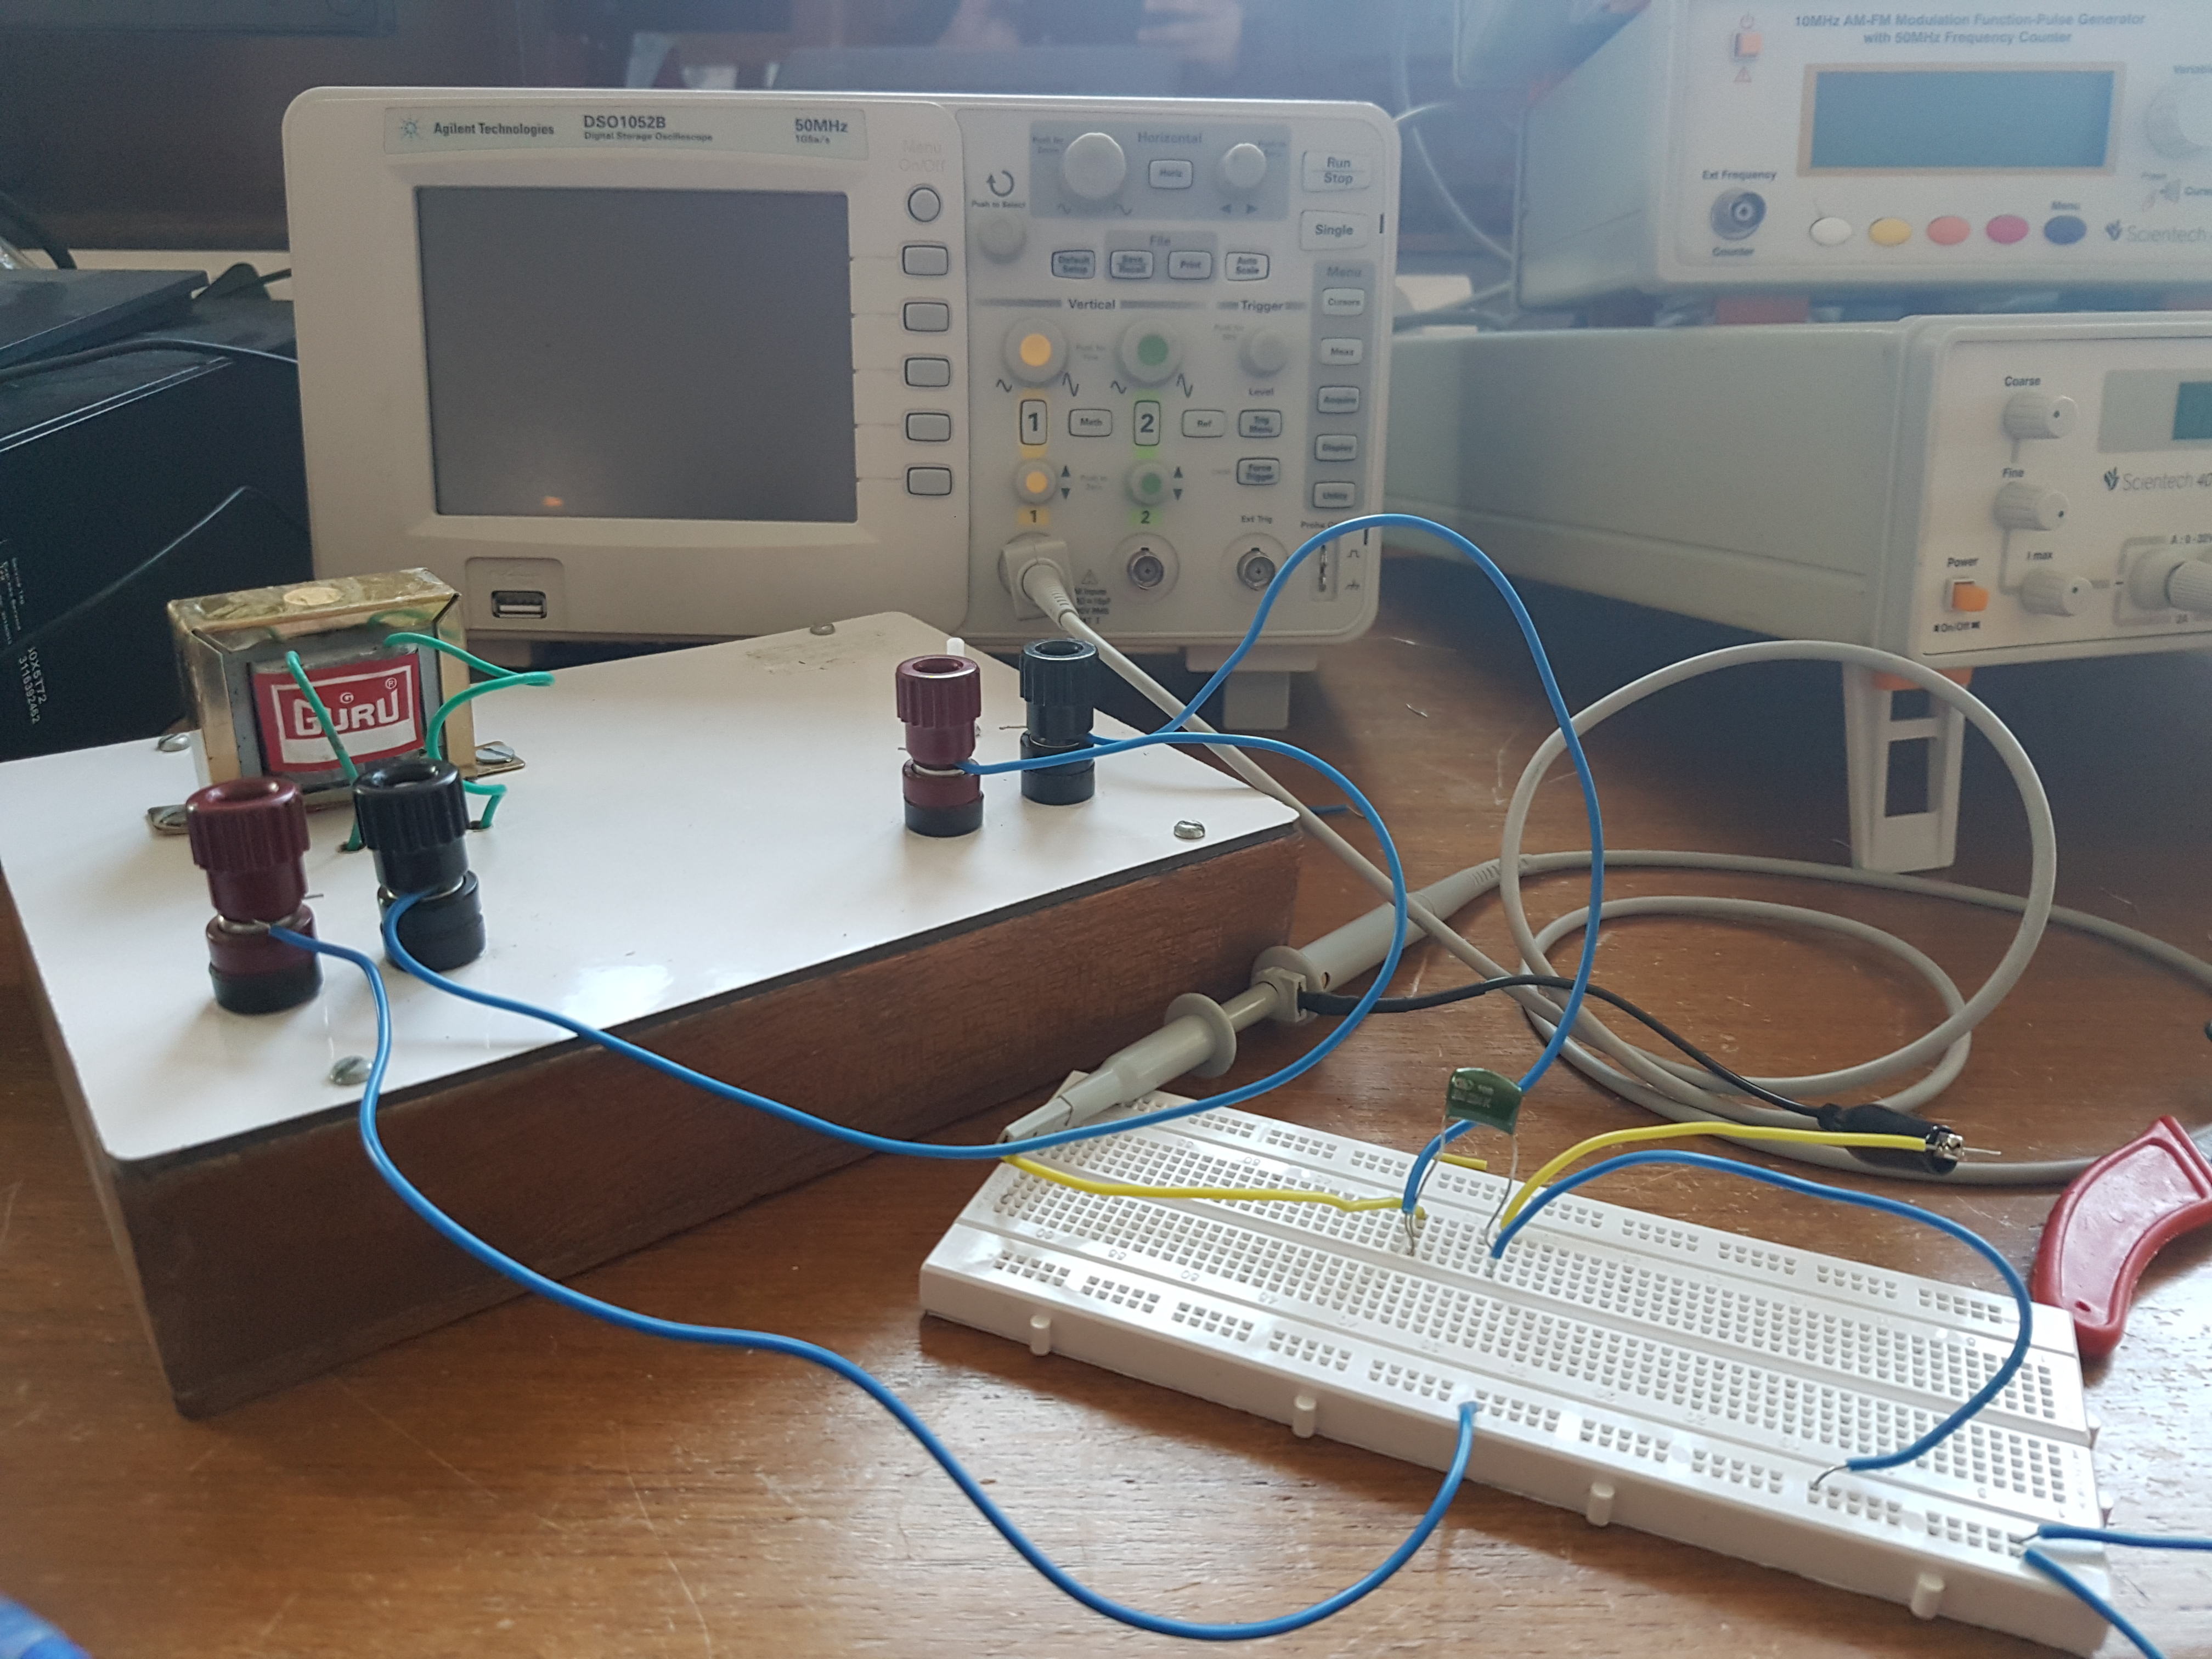
\includegraphics[width=0.9\columnwidth, height=150px]{Circuit2.jpg}}
\end{center}

\subsection{Observation}
\vspace{10px}
\begin{center}
\begin{tabular}{| c | c | c |} 
 \hline
    \ & \ & \ \\
    Resistance($\Omega$) & $\alpha$ & $\omega_0$ \\
    \ & \ & \ \\
    \hline
    \ & \ & \ \\
    500 & 125 & 1507.55 \\
    5800 & 1450 & 1507.55 \\
    10000 & 2500 & 1507.55 \\
    \ & \ & \ \\
    \hline
\end{tabular}
\end{center}
\vspace{10px}
\subsection{Calculation}
\vspace{10px}
For Critically Damped Case, $\alpha=\omega_0$. Thus, R=2L$\omega_0$.

\noindent
Or $R=2\times2\times1507.55 = 6030.2 \Omega$
\vspace{5px}
\subsection{Error Analysis}
Calculated Value of R for Critical Damping= 6.03 k$\Omega$
Measured Value of R for Critical Damping= 5.80 k$\Omega$ 
\vspace{5px}

\noindent
Thus, Error= 0.23k$\Omega$ \\
Error Percentage= $\frac{0.23}{6.03}\times 100 = 3.8 \%$

\newpage

\subsection{Time Domains}
\subsubsection{Under Damped Circuit}
\begin{itemize}
    \item $\Delta V = 4.32V$ (Step Voltage)
    \item $t_d = 800 \mu s$ (Time till it reaches half the Step Voltage)
    \item $t_r = 1.16 ms$ (Time till it reaches Step Voltage First time)
    \item $t_p = 2.12 ms$ (Time till Overshoot Voltage)
    \item $t_s = 11.7 ms$ (Time till deflection from step voltage is $\leq 2\%$)
\end{itemize}

\subsubsection{Critically Damped Circuit}
\begin{itemize}
    \item $t_d = 1 ms$ (Time till it reaches half the Step Voltage)
    \item $t_r = 2.4 ms$ (Time till it reaches Step Voltage First time)
\end{itemize}

\subsubsection{Over Damped Circuit}
\begin{itemize}
    \item $t_d = 1.62ms$ (Time till it reaches half the Step Voltage)
    \item $t_r = 5.2 ms$ (Time till it reaches Step Voltage First time)
\end{itemize}
\vspace{10px}
\begin{center}
\fcolorbox{black}{white}{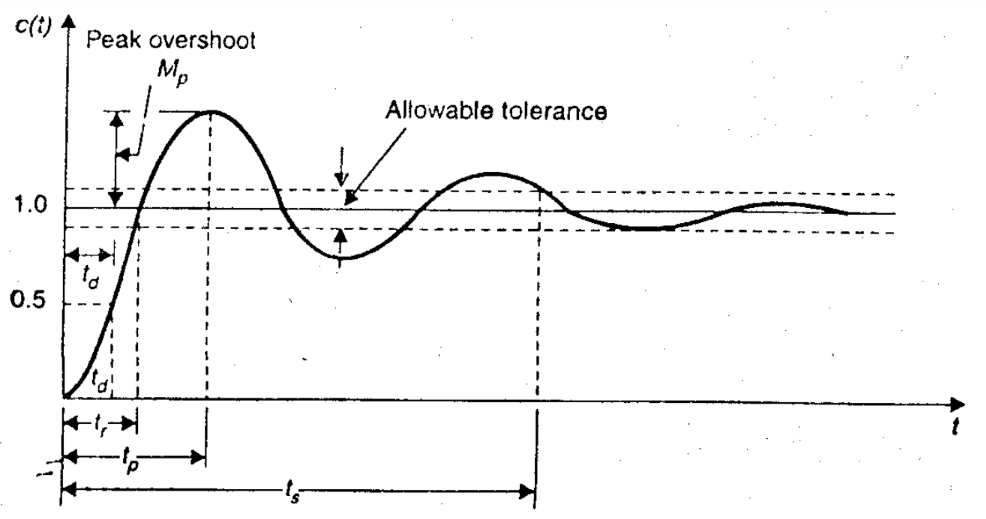
\includegraphics[width=0.9\columnwidth]{Time.png}}    
\end{center}

\newpage

\subsection{DSO Images}
\vspace{5px}
\begin{multicols}{2}
\begin{center}
\fcolorbox{black}{white}{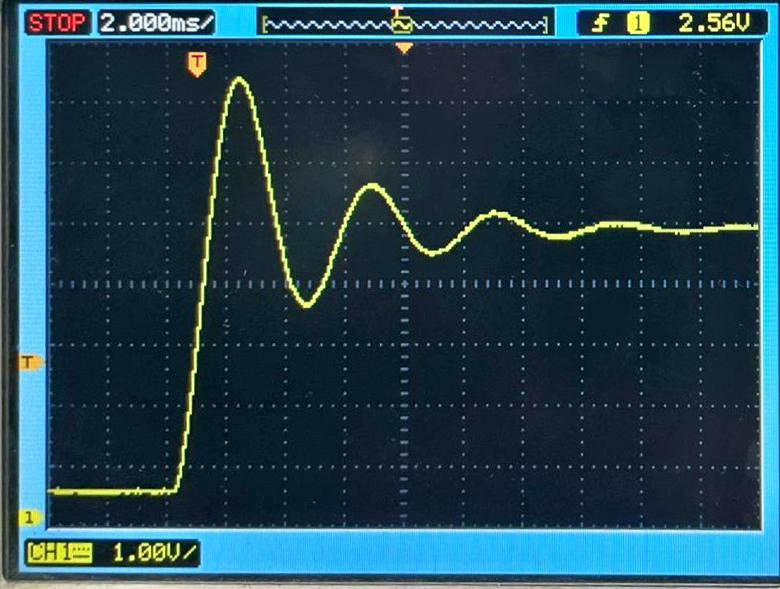
\includegraphics[width=0.9\columnwidth, height=110px]{UnderDamped.jpeg}} \\ \vspace{5px}
Under Damped R=$500\Omega$\\

\columnbreak

\fcolorbox{black}{white}{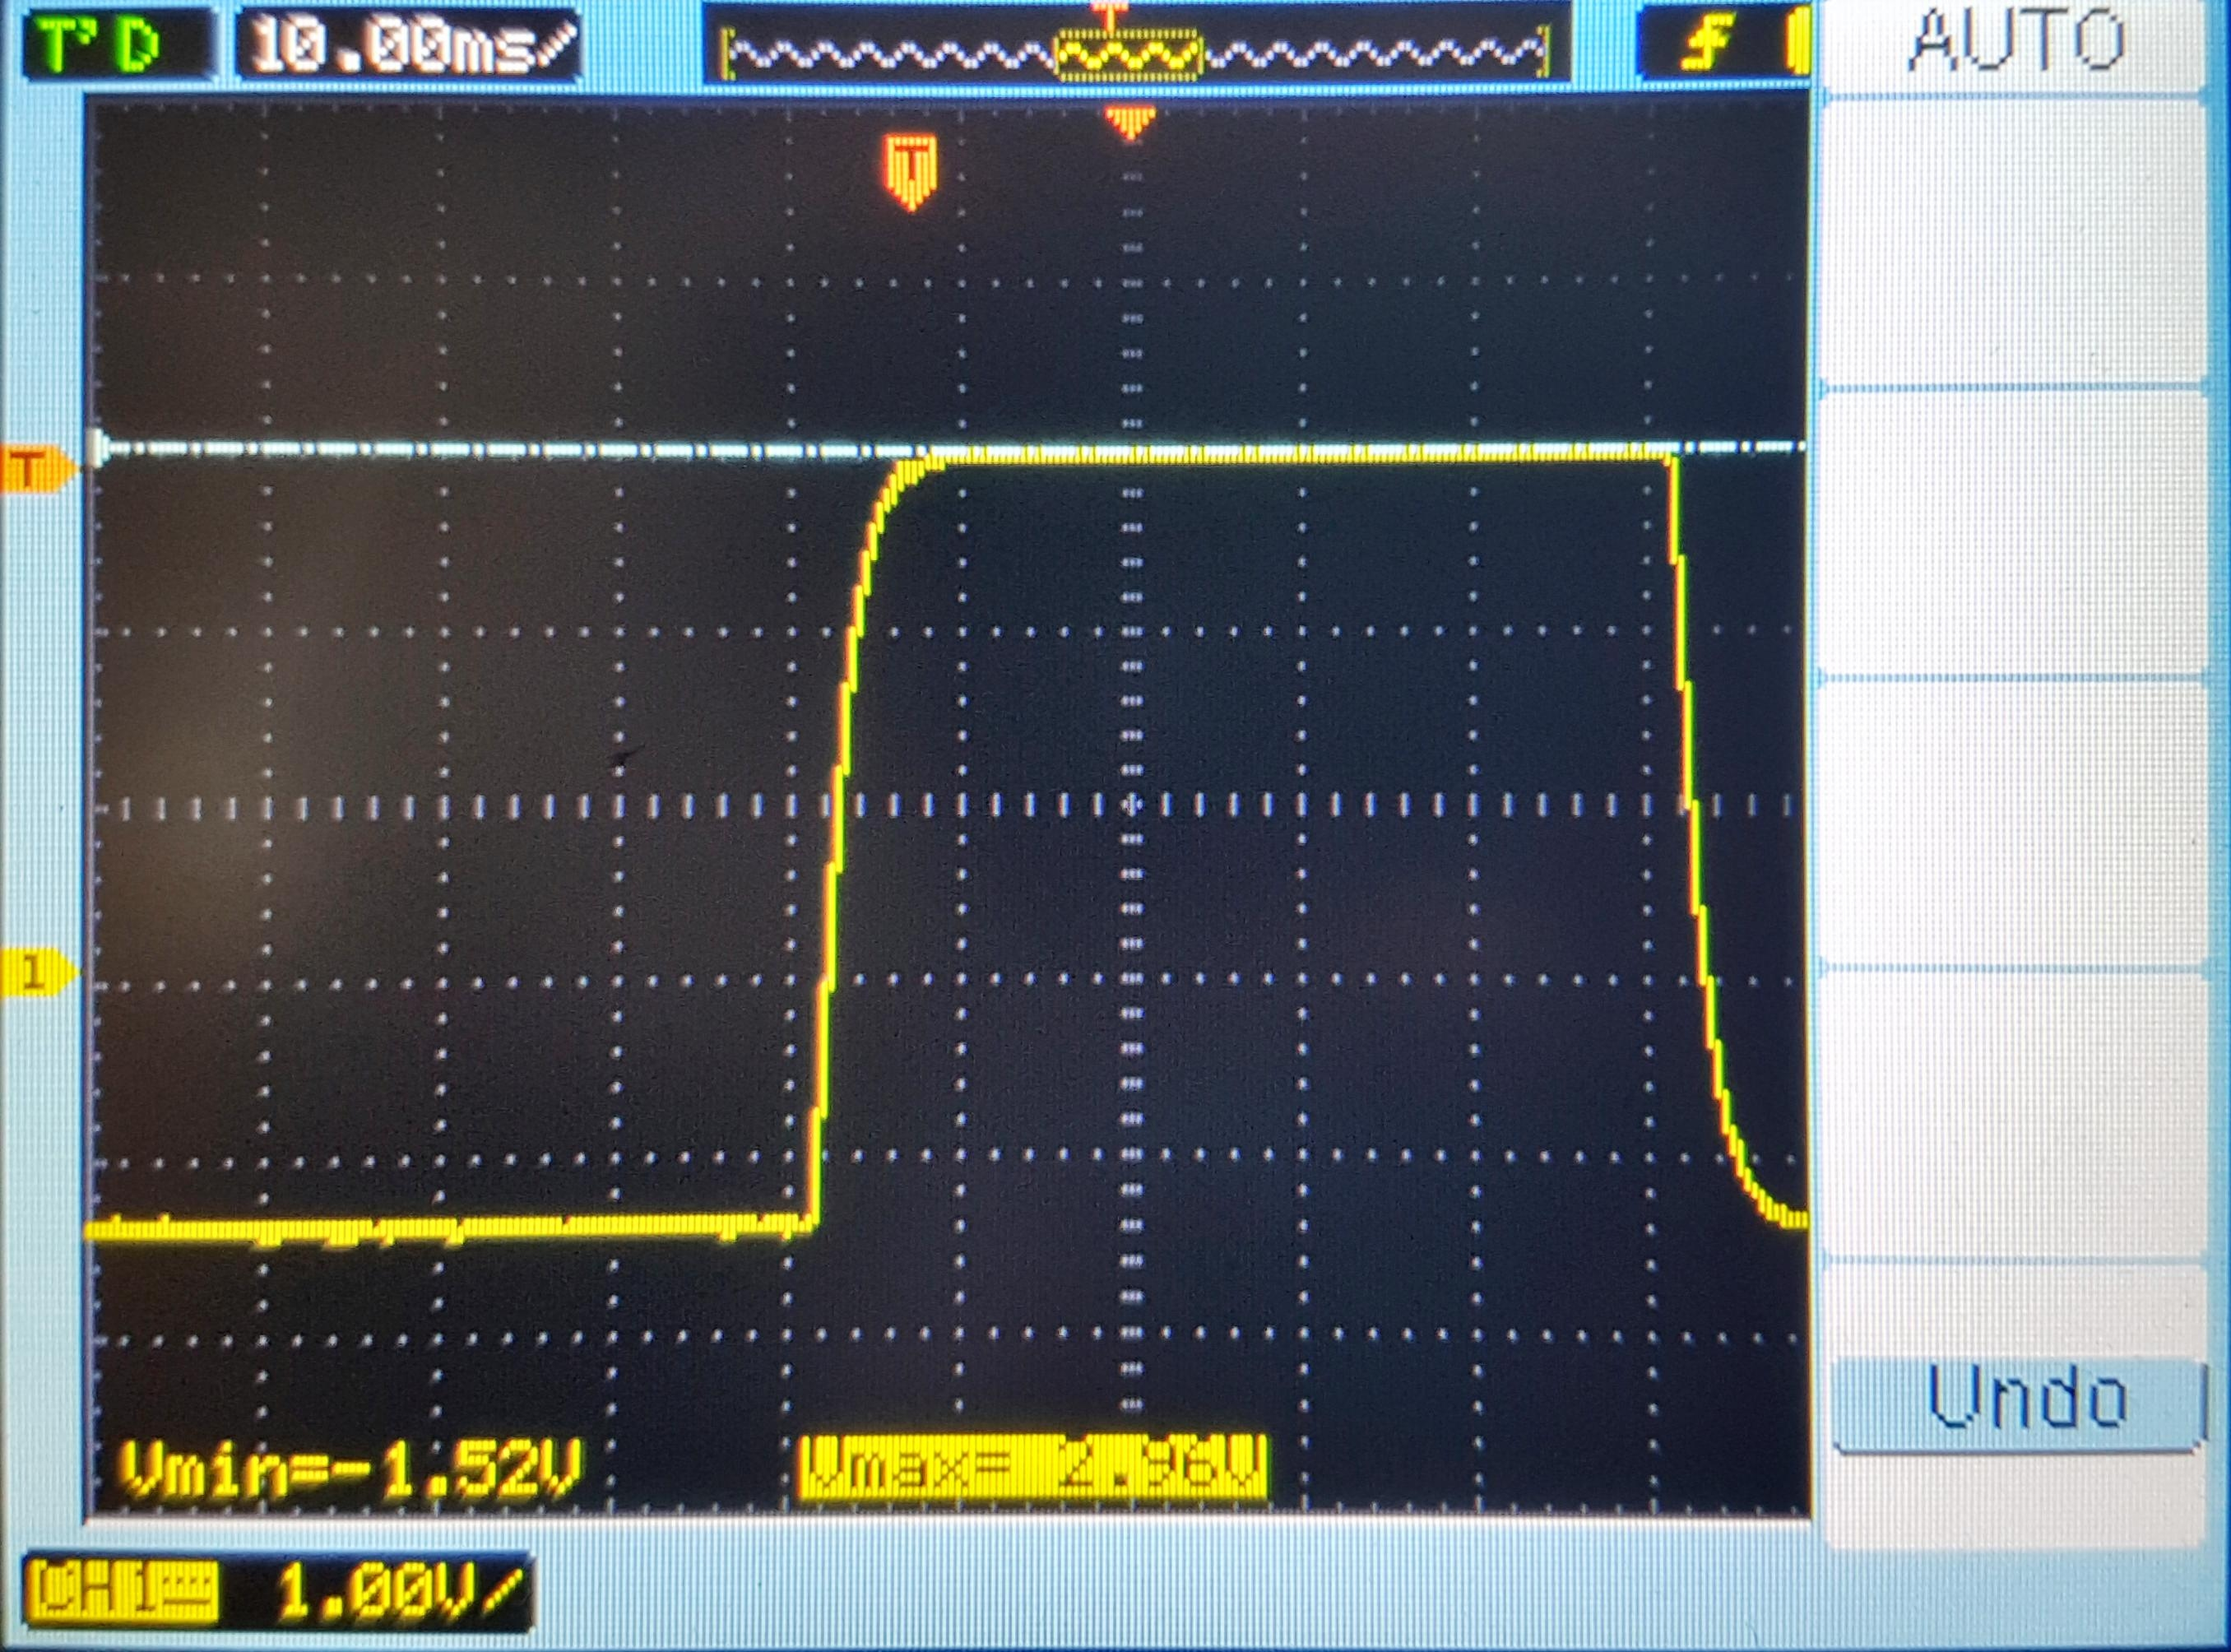
\includegraphics[width=0.9\columnwidth, height=110px]{Critically Damped.jpeg}} \\ \vspace{5px}
Critically Damped R=$5.8k\Omega$
\end{center}
\end{multicols}
\begin{multicols}{2}
\begin{center}
\fcolorbox{black}{white}{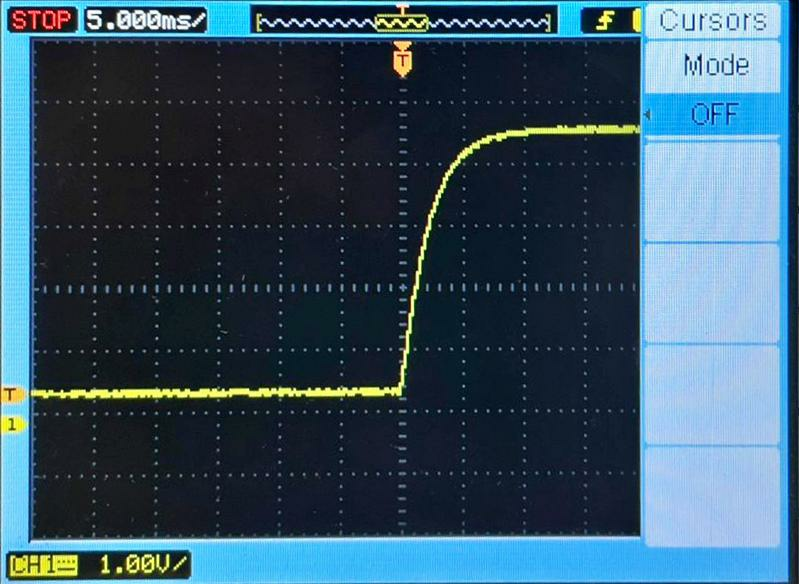
\includegraphics[width=0.9\columnwidth, height=110px]{OverDamped.jpeg}} \\ \vspace{5px}
Over Damped R=$10k\Omega$ \\

\columnbreak

\fcolorbox{black}{white}{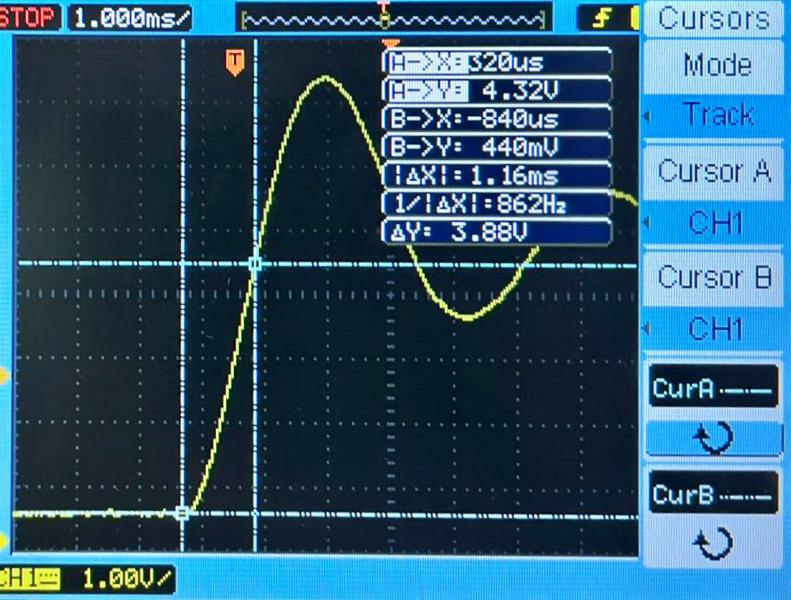
\includegraphics[width=0.9\columnwidth, height=110px]{V Measure.jpeg}} \\ \vspace{5px}
Measurement of Step Voltage in Under Damped Condition
\end{center}
\end{multicols}
\begin{multicols}{2}
\begin{center}
\fcolorbox{black}{white}{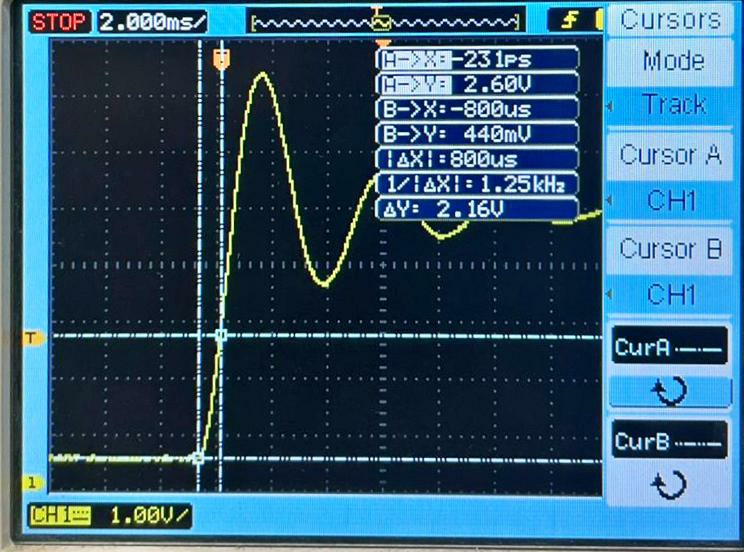
\includegraphics[width=0.9\columnwidth, height=110px]{td.jpeg}} \\ \vspace{5px}
Measurement of $t_d$ in Under Damped Condition \\

\columnbreak

\fcolorbox{black}{white}{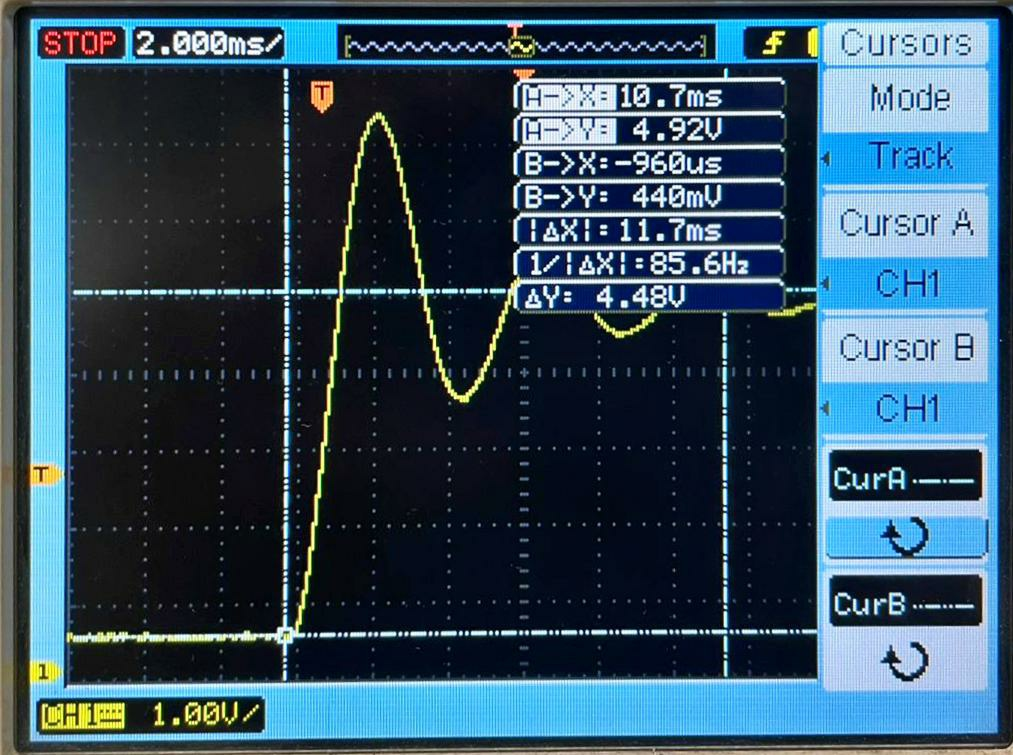
\includegraphics[width=0.9\columnwidth, height=110px]{ts.jpeg}} \\ \vspace{5px}
Measurement of $t_s$ in Under Damped Condition
\end{center}
\end{multicols}

\subsection{Conclusion}
Hence we were able to observe various damping conditions in the step response in a series RLC circuit and were able to measure the different time domain specifications from a DSO apparatus.

\newpage



\section{Sources of Error}
\begin{itemize}
\item Loose connections.
\item Resistance in wires and change due to temperature.
\item Difference in actual resistance, capacitance or inductance from measured value
\item Deviations due to tolerance in values
\item Connections changed while circuit is powered.
\end{itemize}

\vspace{15px}

\section{Precautions}

\begin{itemize}
\item Insulated tools should be used.
\item Electric wires (jumpers) should be properly snipped.
\item Proper shoes should be worn.
\item Circuit should not be left powered for long time.

\end{itemize}

\vspace{15px}

\section{Concluding Remarks}
In this experiment, we verified the concepts of step response in series RC and LCR circuits. In the first part of the experiment, we obtained the value of time constant from the graph shown on the DSO screen. The values were roughly equal to the theoretical values with a deflection of nearly 18.7 \%. This is within experimental errors. In the second part of the experiment we got to know how different types of damping can be observed in a series LCR circuit. We also showed these cases valid for under damped, over damped and critically damped conditions. We also verified the value of resistance for achieving critically damped case came close to the theoretical value with a deflection of nearly 4 \%. We also found out the various time domain specifications from the graphs obtained on the DSO screen.
\end{document}
